\documentclass[12 pt, a4paper]{article}% тип документа, размер шрифта
\usepackage{cmap}	
\usepackage{hyperref}
\hypersetup{
	colorlinks=true,
	linkcolor=blue,
	urlcolor=blue,
}
\usepackage{mathtext}
\usepackage[T2A]{fontenc}%поддержка кириллицы в ЛаТеХ
\usepackage[utf8]{inputenc}%кодировка
\usepackage[english,russian]{babel}
\usepackage{indentfirst}

\usepackage{amsmath,amsfonts,amssymb,amsthm,mathtools} % AMS
\usepackage{amsmath}%удобная вёрстка многострочных формул, масштабирующийся текст в формулах, формулы в рамках и др.
\usepackage{amsfonts}%поддержка ажурного и готического шрифтов — например, для записи символа {\displaystyle \mathbb {R} } \mathbb {R} 
\usepackage{amssymb}%amsfonts + несколько сотен дополнительных математических символов
\frenchspacing%запрет длинного пробела после точки
\usepackage{setspace}%возможность установки межстрочного интервала
\usepackage{indentfirst}%пакет позволяет делать в первом абзаце после заголовка абзацный отступ
\onehalfspacing%установка полуторного интервала по умолчанию
\usepackage{graphicx}%подключение рисунков
\graphicspath{{images/}}%путь ко всем рисункам
\usepackage{caption}
\usepackage{float}%плавающие картинки
\usepackage{tikz} % это для чудо-миллиметровки
\usepackage[export]{adjustbox}
\usepackage{pgfplots}%для построения графиков
\pgfplotsset{compat=newest, y label style={rotate=-90},  width=10 cm}%версия пакета построения графиков, ширина графиков
\usepackage{pgfplotstable}%простое рисование табличек
\usepackage{lastpage}%пакет нумерации страниц
\usepackage{comment}%возможность вставлять большие комменты
\usepackage{float}
%%%%% ПОЛЯ
\setlength\parindent{0pt} 
\usepackage[top = 2 cm, bottom = 2 cm, left = 1.5 cm, right = 2 cm]{geometry}
\setlength\parindent{0pt}
%%%%% КОЛОНТИТУЛЫ
\usepackage[shortlabels]{enumitem}

\usepackage{array,tabularx,tabulary,booktabs} % Дополнительная работа с таблицами
\usepackage{longtable} % Длинные таблицы
\usepackage{multirow} % Слияние строк в таблице
\usepackage{colortbl} % Цветная заливка в таблице
\usepackage[labelsep=period,labelfont=rm,tablename={Таблица},tablewithin=none]{caption}
\usepackage{makecell} 
\usepackage{ctable} % for \specialrule command 

\usepackage{fancybox, fancyhdr}
\pagestyle{fancy} 
\fancyhead[L]{\textit{6 класс}}
\fancyhead[C]{\textit{{ЛМШ "Алые паруса" 2023}}}
\fancyhead[R]{\textit{2 день}} % ЛЮБАЯ ДОПОЛНИТЕЛЬНАЯ ИНФОРМАЦИЯ
%\fancyfoot[R]{Задание с двух сторон!}
\renewcommand{\footrulewidth}{0.3 mm}

\usepackage{tikzsymbols}
\usepackage{textcomp}
\usepackage{parskip}
\usepackage{graphicx}
\graphicspath{{pictures/}}
\DeclareGraphicsExtensions{.pdf,.png,.jpg}
\usepackage{wrapfig}
%%% Заголовок

%%% Новые команды
\newcommand{\z}[1]{{{\vspace{0.6cm} \large\textbf{{Задача {#1}} \\ }}}}
\newcommand{\task}[1]{{{\vspace{0.6cm} \vspace{-2ex} \textbf{№{#1}} }}}
\newcommand{\otv}{{\vspace{0.3cm} \textbf{Решение: } \\}}
\newcommand{\uk}{\underline{\textit{Указание.}} }
\newcommand{\opr}{\textit{Определение: }}
\newcommand{\sol}[1]{{{\vspace{0.3cm} \textbf{{Задача {#1}} }\\ }}}
\newcommand{\RomanNumeralCaps}[1]
{\MakeUppercase{\romannumeral #1}}

\usepackage{cancel}
\usepackage{epigraph} 
\setlength\parindent{0pt}
\setlength\parskip{1ex plus 2pt minus 1pt}
\newcommand\X{\par\noindent---~}
\usepackage{ upgreek }
\begin{document} % конец преамбулы, начало документа
	\newpage
	\begin{flushright}
		\textit{<<Чёрт знает, чем всё кончится, но хорошо, что хоть начинается.>>}
	\end{flushright}
	\begin{figure}[t]
		\begin{minipage}[h]{0.33\linewidth}
			
\includegraphics[width=0.33\linewidth, left]{logo.jpg}
		\end{minipage}
		%%	\hfill
		\begin{minipage}[h]{0.33\linewidth}
			\centering
			\large{\textbf{ОТВЕТЫ НА ВСТУПИТЕЛЬНУЮ РАБОТУ}}\\
		\end{minipage}
		\begin{minipage}[h]{0.33\linewidth}
			
\includegraphics[width=0.33\linewidth, right]{logo.jpg}
		\end{minipage}
		\label{ris:image1}
	\end{figure}
	\begin{comment}
			\begin{figure}[b]
		\begin{minipage}[h]{0.33\linewidth}
			
\includegraphics[width=0.33\linewidth, left]{logo.jpg}
		\end{minipage}
		%%\hfill
				\begin{minipage}[h]{0.33\linewidth}
			\centering
			\large{\textbf{ЕСЛИ ПОЯВИЛИСЬ ВОПРОСЫ, ТО ОБЯЗАТЕЛЬНО ЗАДАВАЙТЕ ИХ}}\\
		\end{minipage}
		\begin{minipage}[h]{0.33\linewidth}
			
\includegraphics[width=0.33\linewidth, right]{logo.jpg}
		\end{minipage}
		\label{ris:image1}
	\end{figure}
	\end{comment}
	\begin{comment}
		\begin{tabular}{lcr}
			
\includegraphics[width=0.2\linewidth]{logo.jpg} &
			\vspace{-2ex}
			\large\textbf{Вступительная работа} &
			
\includegraphics[width=0.2\linewidth]{logo.jpg}
		\end{tabular}
	\end{comment}
	\raggedright
	
	\task{1} $1,5 \div \frac{13}{19} - (1,5 + \frac{13}{19}) = \frac{2}{247}$  $\longrightarrow$ $1,5 \div \frac{13}{19} > 1,5 + \frac{13}{19}$\\
	
	\task{2}$((1 \cdot 3 \cdot 3 \cdot 3) + 3 + 3) \div 3 = 11$ или $(1 \cdot 3 + 3) \div 3 + 3 + 3 + 3 = 11$ \\
	
	\task{3}  Пример решения снизу(см. рис. 1). Также существуют другие варианты.

	\task{4} 24 кг никеля, 32 кг цинка, 104 кг меди\\
	
	\task{5} 160 км	\\
	
	\task{6} $x \in [-3, 3]$ $\longrightarrow$ ответ: $\{-3, -2, -1, 0, 1, 2, 3\}$\\
	
	\task{7} $2 \cdot 2 \cdot 2 = 8$, в 8 раз после семи стирок уменьшился объем мыла.\\
	Следовательно у Лины осталась $\frac{1}{8}$ изначального куска мыла.\\
	$1 - \frac{1}{8} = \frac{7}{8}$ мыла использовали.\\
	$\frac{7}{8} \div 7 = \frac{1}{8}$ объема мыла тратится за одну стирку.\\
	Значит, остатка мыла хватит на одну стирку.\\
	
	\task{8} На одной горизонтали не может стоять больше одной ладьи — иначе они будут бить друг друга. Значит, ладей можно поставить не больше, чем горизонталей у доски, а их 8. Следовательно, больше 8 ладей поставить на доску нельзя.\\
	
	\task{9} Найдём сумму чисел по всем столбцам $S_{столб} = m \cdot 100$.\\
	Найдём сумму чисел по всем строкам $S_{строк} = n \cdot 100$.\\
	Сумма всех чисел в таблице не меняется от методики подсчёта, значит $S_{столб} = S_{строк}$, следовательно $m \cdot 100 = n \cdot 100$, тогда $m = n$.\\
	
	\task{10} Клетки квадрата $10 \times 10$ раскрасим в 4 цвета, так, чтобы любой прямоугольник $1 \times 4$, занимал 4 разных цвета (см. рис. 2). Если нам удасться разрезать квадрат на прямоугольники, то всех цветов в квадрате будет поровну. Но (не трудно сосчитать) в нашем квадрате цветов не поровну. А именно клеток с цветом 1 ‑ 26, 2 – 25, 3 – 24, 4 – 25. Значит квадрат $10 \times 10$ нельзя разрезать на прямоугольники $1 \times 4$.\\
	
	\begin{figure}[H]
		\begin{minipage}[h]{0.5\linewidth}
			\centering
			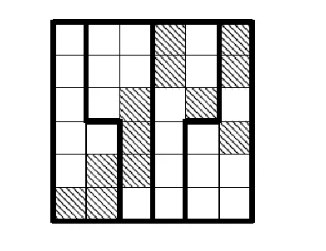
\includegraphics[width=0.75\textwidth]{6_ans_1.jpg}
		\end{minipage}
		\hfill
		\begin{minipage}[h]{0.5\linewidth}
			\centering
			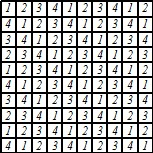
\includegraphics[width=0.5\textwidth]{10_ans.jpg}
		\end{minipage}
	\end{figure}
\end{document} 